%!TEX root = ./rules-working.tex
%LTeX: enabled=true

\rulechapter{Maritime Operations}

\label{rule:naval-units}

\section{The Sea}

The sea is always considered to be flat terrain at altitude zero. 

Scenarios may specify that the sea is in one of three sea states: Calm, Moderate, or Heavy.   

When calm seas are in effect, aircraft with limited look-down technology are considered to have full look-down capability for the purposes of radar search and lock-on of air targets over the sea, while aircraft with no look-down technology are considered to have limited look-down capability.  

When heavy seas are in effect, +1 is added to all air-to-sea attacks and to ASM hits (Table \ref{table:asm-hits}) rolls (but not to ASM to-hit rolls)\addedin{3A}{3A-ship-movement}{\ and all ships' maximum speeds are half the value given in the Ship Data Table}.  

Moderate seas do not give any bonuses or penalties to radar or combat.

When moderate or heavy seas are in effect, the scenario must specify the wind direction.  This affects the use of decoys (see rule \ref{rule:asm-decoys}).

\paragraph{Radar Horizon.} 

Because the sea is essentially flat, the radar horizon primarily depends on the height of the EWR above the water surface.  Heavy sea state can affect smaller ships because of wave heights and rolling of the radar beam, reducing the effective range of the radar.  Aircraft in TFF and ASM SS or SS+ missiles may be detected by ships with MTI capable EWR or “T” level capable SAMs having a line of sight to them. Table~\ref{table:radar-horizon} sets out the detection ranges in hexes.


\begin{twocolumntablefloat}
\begin{twocolumntable}
\tablecaption{table:radar-horizon}{Radar Horizon.}
\begin{tabularx}{0.7\linewidth}{lCC}
\toprule
Class Type&EWR Range TFF&EWR Range SS, SS+\\
\midrule
CV, CVN, BB	          &120	 &90\\
BGCN, CVL, LSD	      &100	 &70\\
CGN, CG, CA           &90/80 &60/50\\
CL, DDG, DD, DDH, LST &80/70 &60/40\\
FFG, FF, FFL	      &70/50 &50/20\\
FAC                   &60/40 &30/10\\
\bottomrule
\end{tabularx}
\end{twocolumntable}

\medskip

\begin{tablenote}{0.7\linewidth}
Range after a slash, if any, is the range in Heavy sea state. AEGIS ships do not lose effectiveness in Heavy sea state.
\end{tablenote}
\end{twocolumntablefloat}

\section{Naval Targets}

Naval vessels are special targets whose characteristics are given in the Ship Data Tables rather than on their counters.  Ship counters always represent single sea vessels and must be faced\deletedin{3A}{3A-ship-facing}{, as for aircraft}.  Most ships are classified as warships, though some may be given other classifications such as fleet auxiliary, tanker, or transport.

\paragraph{Ship Data Charts}
The Ship Data Tables list the characteristics and values for each class of ship as follows: 

\begin{itemize}

    \itemaddedin{3A}{3A-ship-movement}{\itemparagraph{Size and Type.} Ships are classified as large, medium, or small and as warships or merchant ships. The maneuverability of a ship depends on its size and type.}
    
    \itemaddedin{3A}{3A-ship-movement}{\itemparagraph{Maximum Speed.} The ship's maximum speed in knots in calm or moderate seas. The ship's maximum speed is half the value given.}

    \item \itemparagraph{VP.} Victory Point values are listed as three figures.  The first is the points awarded at the end of the game for each point of damage to an uncrippled ship; the second is the point value awarded for crippling a ship; and the third is the points awarded for sinking a ship.

    \item \itemparagraph{Defense Strength.} Treated the same as land targets.

    \item \itemparagraph{Spotting Range.} Treated the same as land targets.
    
    \item \itemparagraph{Hull.} The first figure is the Hull Value.  If the amount of damage a ship takes equals this value, it is crippled; and if more it is sinking. The second figure is the Sinking Number used once a scenario is over to determine whether a sinking vessel actually sinks.

    \item \itemparagraph{Jam.} This value represents the capabilities of the ship's radar deception and break-lock jammers used to defeat ARH ASMs.

    \item \itemparagraph{Decoy.} This represents the value of the ship's decoy launchers.  If two numbers are listed, separated by a slash, the first is the effectiveness versus ARH ASMs and the second is the effectiveness against IRH ASMs.

    \item \itemparagraph{Radars.} Ship's radars are listed separately by type and frequency. All radars are elevated unless otherwise indicated.

    EWRs may pass down radar contacts to all on-board TTRs.  This section notes whether the radar has MTI capability. TTRs list their range in megahexes (mh) as well as noting any Quick Reaction or Multi-Target Engagement capability.  Unless listed as being part of a specific SAM system, TTRs provide tracking for all SAMs on board, regardless of the number of launchers.

    FCRs, if any, specify the gun system they are attached to.

    \item \itemparagraph{Gun Directors.} This shows the maximum range (as a multiple of aircraft size in hexes) that ship's AAA can engage aircraft and missiles/rockets without radar direction.  If no gun director value is given, use the visual range criteria given for land-based AAA in Rule 24.3.

    \item \itemparagraph{AAA} This lists the number and values of all AAA sites on board the ship. 

    \item \itemparagraph{SAM} This lists the number of SAM launchers and the values for each launcher.  Note that in most cases, multiple launchers will use the same TTR and may not launch at separate targets unless that TTR has Multi-Target Engagement (ME) capability.

    AAA and SAMs may have arc limitations listed in the Ship Data Tables. Heavy AAA does not have to keep track of facing, but may only fire into the ship arcs listed.  SAMs may launch missiles at any target, regardless of arc, but the missile's initial facing must be within the listed arc.  An arc notation of “All” means there is no limitation.
\end{itemize}

\changedin{3A}{3A-ship-movement}{

\paragraph{Ship Movement.} 

Ships may move on those turns specified by the scenario. Generally, warships can move one hex every other turn and merchants, tankers, and cargo ships can move one hex every fifth or sixth turn. They move at the end of the Flight Phase after all movement and ground/sea attacks are complete; they may only move one hex and must move directly ahead, as for aircraft.  Ships may not move onto hex-sides.  Unless otherwise specified, ships may always alter their heading by 30° every Flight Phase they are able to move, just before any forward movement takes place.  Warships (only) under Cruiser size may alter their heading up to 60° instead, but if they elect to do so they may not fire AAA or launch and/or guide SAMs in the following game turn.

}{

\paragraph{Ship Movement Phase.}

Actions related to ships' movement occur in the Ship Movement Phase, immediately after the Ground Unit Interactions phase. In the Ship Movement Phase:
\begin{enumerate}
\item A ship must move forward one hex if the number of game turns since it last did so (or since the start of the game if it has not yet done so), including the current game turn, is equal to or more than its current move cadence (defined below).

\item A ship may complete a turn if the number of game turns since it declared the turn is equal to or more than its current turn cadence. When a ship completes a turn, it changes facing by 60 degrees in the declared direction.

\item A ship may abort a previously declared turn.

\item A ship may declare a turn, indicating its direction and whether it is a normal turn or a hard turn.

\item A ship may increase or decrease its speed, within to the limits defined below, and calculate its new move and turn cadences.

\end{enumerate}
These actions must be carried out in this order.

%!TEX root = ./rules-working.tex
%LTeX: enabled=true
\begin{twocolumntablefloat}
\addedin{3A}{3A-ship-movement}{

\tablecaption{table:ship-movement}{Ship Movement and Turning.}
    
\begin{tabularx}{0.7\linewidth}{llCCCCC}
\toprule
Type&Size&\multicolumn{2}{c}{Maximum}&Maximum&\multicolumn{2}{c}{Turn}\\
&&\multicolumn{2}{c}{Speed}&Speed&\multicolumn{2}{c}{Cadence}\\
&&\multicolumn{2}{c}{Increase}&Decrease&\multicolumn{2}{c}{Numerator}\\
\cmidrule{3-4}
\cmidrule{6-7}
&&Up to 1/2 Max Speed&1/2 Max Speed or More&&Normal&Hard\\
\midrule
Warship       & Large  & 0.5 & 0.25\phantom{} & 1.0 & \phantom{0}80 & \phantom{0}60 \\
              & Medium & 1.0 & 0.5\phantom{0} & 1.5 & \phantom{0}60 & \phantom{0}40 \\
              & Small  & 1.0 & 0.5\phantom{0} & 1.5 & \phantom{0}40 & \phantom{0}20 \\
Merchant Ship & Large  & 0.5 & 0.25\phantom{} & 0.5 & \phantom{}160 & \phantom{}140 \\
              & Medium & 0.5 & 0.25\phantom{} & 0.5 & \phantom{}160 & \phantom{}100 \\
              & Small  & 0.5 & 0.25\phantom{} & 0.5 & \phantom{0}80 & \phantom{0}60 \\
\bottomrule
\end{tabularx}

\smallskip

\begin{tablenote}{0.7\linewidth}
    \small
    \begin{itemize}
        \item The maximum speed increase or decrease are in knots per game turn. 

        \item The move cadence of a ship is 87 divided by its speed in knots and rounded to the nearest integer with halves rounded up. A ship must move forward one hex if the number of game turns since it last did so (or since the start of the game if it has not yet done so), including the current game turn, is equal to or more than its current move cadence.
        
        \item The turn cadence of a ship is the turn cadence numerator, from the table, divided by its speed in knots and rounded to the nearest integer with halves rounded up. A ship may complete a turn if the number of game turns since it declared the turn, including the current game turn, is equal to or more than its current turn cadence. When a ship completes a turn, it changes facing by 60 degrees in the declared direction. A ship must have and maintain at least 5 knots for a normal turn and 10 knots for a hard turn. A turning ship may not increase its speed. 
        
        \item An anchored ship always has a speed of 0 knots and may not move or turn. A crippled ship may not increase its speed, must decrease its speed at half the maximum rate until it reaches 0 knots, and may not turn.

    \end{itemize}
\end{tablenote}

}
\end{twocolumntablefloat}


\paragraph{Ship Speed.} 

Ships speeds are measured in knots, with 1 knot being approximately 1.15 mph. During the Ship Movement Phase, a ship may declare a new speed. The limits on the new speed depend on the size and type of ship, its current speed, whether it is turning, anchored, or crippled.

If a ship is not turning, anchored, or crippled, it may increase its speed according to Table~\ref{table:ship-movement}. A ship may not increase its speed beyond its maximum speed for the sea state. 

A ship may decrease its speed according to Table~\ref{table:ship-movement}. A crippled ship must decrease its speed at half the maximum rate. A ship may not decrease its speed below 0 knots.

For example, HMS {\itshape Arrow}, a small warship with a maximum speed of 30 knots, is in moderate seas and is neither anchored nor crippled.
\begin{itemize}

    \item If it has current speed of 24.0 knots and does not turn, it may declare a new speed between 22.5 and 24.5 knots. If it turns, it may declare a new speed between 22.5 and 24.0 knots.

    \item If it has a current speed of 12.0 knots and does not turn, it may declare a new speed between 10.5 and 13.0 knots. If it turns, it may declare a new speed between 10.5 and 12.0 knots.

\end{itemize}

\paragraph{Ship Moves.}

The game scale has 100 mph or 87 knots corresponding to 1 hex per game turn. Since ships are slower than this, they do not move every game turn, but instead move one hex after accumulating game turns equal to or more than their current \emph{move cadence}. The count starts on the first game turn and is reset each time the ship moves one hex. A ship's move cadence is 87 divided by its speed in knots and rounded to the closest integer, with halves rounded up. 

For example, HMS {\itshape Arrow} is moving at 20 knots and has a move cadence of 4 (as 87/20 is 4.35 which rounds to 4). It will move forward one hex every four game turns.

\paragraph{Ship Turns.}

When a ship declares a turn, it indicates the direction and whether it is a \emph{normal} turn or a \emph{hard} turn.

Turning requires a ship must have and maintain sufficient steerage way. A ship must have a speed of at least 5 knots to declare a normal turn and must maintain this speed until the turn is completed. For a hard turn, it must have and maintain a speed of 10 knots. If it does not maintain the required speed, the turn is implicitly aborted. 

Ships may complete a turn and change facing by 60 degrees after accumulating game turns equal to their \emph{turn cadence}. The count starts when the turn is declared. A ship's turn cadence is the turn cadence numerator from Table \ref{table:ship-movement} for the ship type and size and the type of turn divided by its speed in knots and rounded to the closest integer, with halves rounded up. The change of facing occurs in place; unlike aircraft and missiles, a ship does not have to move to change facing.

During a hard turn, a ship may not perform AAA attacks of any kind or launch SAMs, and any SAMs being guided by the ship lose track. These restrictions apply from the moment a hard turn is declared to the end of the Ship Movement Phase of the game turn after it is completed or aborted.

Turns may be aborted and stretched out. 

When a ship completes a turn, it must change facing by 60 degrees in the declared direction. Changing facing by 30 degrees is not allowed. A ship must always face towards an adjacent hex, must not face towards adjacent hex-sides, and must not move onto a hex-side.

%!TEX root = ../rules-working.tex
%LTeX: enabled=false

\begin{twocolumnfigure}[tp]
\addedin{3A}{3A-ship-movement}{

\begin{fitheight}{4.4\standardhexwidth}

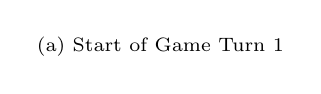
\begin{tikzpicture}
    \setfiguresize{-2.4}{-1.6}{+1.6}{+2.8}
    \drawhexgrid{-2}{-1}{4}{3}
    \drawshipcounter{0.0}{-0.0}{90}{}{}
    \miniathex{-0.5}{+2.20}{\node [anchor=south] {\scriptsize (a) Start of Game Turn 1};}
\end{tikzpicture}

\hspace{5mm}

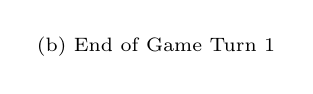
\begin{tikzpicture}
    \setfiguresize{-2.4}{-1.6}{+1.6}{+2.8}
    \drawhexgrid{-2}{-1}{4}{3}
    \drawshipcounter{0.0}{-0.0}{90}{}{}
    \miniathex{-0.5}{+2.20}{\node [anchor=south] {\scriptsize (b) End of Game Turn 1};}
\end{tikzpicture}

\hspace{5mm}

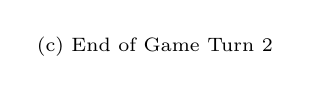
\begin{tikzpicture}
    \setfiguresize{-2.4}{-1.6}{+1.6}{+2.8}
    \drawhexgrid{-2}{-1}{4}{3}
    \drawshipcounter{0.0}{-0.0}{150}{}{}
    \miniathex{-0.5}{+2.20}{\node [anchor=south] {\scriptsize (c) End of Game Turn 2};}
\end{tikzpicture}

\hspace{5mm}

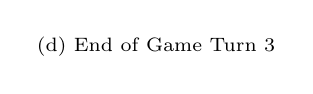
\begin{tikzpicture}
    \setfiguresize{-2.4}{-1.6}{+1.6}{+2.8}
    \drawhexgrid{-2}{-1}{4}{3}
    \drawshipcounter{0.0}{-0.0}{150}{}{}
    \miniathex{-0.5}{+2.20}{\node [anchor=south] {\scriptsize (d) End of Game Turn 3};}
\end{tikzpicture}

\hspace{5mm}

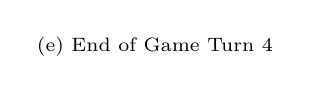
\begin{tikzpicture}
    \setfiguresize{-2.4}{-1.6}{+1.6}{+2.8}
    \drawhexgrid{-2}{-1}{4}{3}
    \drawshipcounter{-1.0}{0.5}{210}{}{}
    \miniathex{-0.5}{+2.20}{\node [anchor=south] {\scriptsize (e) End of Game Turn 4};}
\end{tikzpicture}

\end{fitheight}

\figurecaption{figure:ship-movement-example}{The position of HMS {\itshape Arrow} during the ship movement example in the text.}

}
\end{twocolumnfigure}

For example, HMS {\itshape Arrow}, a small warship, has a current speed of 20 knots. It could move and turn over the first four game turns of a scenario as follows:
\begin{itemize}
\item Game Turn 1:  It declares a hard turn to port. It may not increase speed as it is turning, but maintains 20 knots in this and subsequent game turns. Its move cadence is 4 (as $87/20 = 4.35$ which rounds to 4) and its turn cadence is 1 (as $20/20 = 1$).
\item Game Turn 2: It completes the turn declared on game turn 1 and changes facing by 60 degrees to port (without moving forward). It then declares a normal turn to port. Its turn cadence is 2 (as $40/20 = 2$). It 
\item Game Turn 3: It continues the turn declared on game turn 2.
\item Game Turn 4: It moves forward one hex, and then completes the turn declared on game turn 2 and changes facing by 60 degrees to port.
\end{itemize}
Figure \ref{figure:ship-movement-example} shows these moves and turns. Because of the hard turn declared during game turn 1, {\itshape Arrow} cannot perform AAA attacks or launch or guide SAMs on game turns 2 or 3, but it can on game turns 1 and 4.


\paragraph{Stopped Ships.} A stopped ship is one with a speed of 0 knots and that is neither anchored not crippled. It may not move or turn while stopped, but may increase its speed normally. Once its speed is more than 0 knots, it is no longer stopped and may move and turn normally.

\paragraph{Anchored Ships.} An anchored ship has a speed of 0 knots and may not increase its speed, move, or turn.

\paragraph{Crippled Ships.} A crippled ship may not increase its speed, must decrease its speed at exactly half the maximum rate until its speed is 0 knots, and may not turn.

}

\paragraph{Command Vessels.}

Designated command ships have data\-links with friendly ships. If a command vessel detects a target with its EWR, all friendly ships with a line of sight to the target automatically detect it also.

\paragraph{AEGIS.}

All AEGIS capable ships are considered command ships.   AEGIS EWRs passdown to their TTRs on a roll of 9 or less.  In addition, they may passdown to any friendly ship equipped with the SM-2 MR or SM-3 missile on a roll of 8 or less.  AEGIS vessels may illuminate air targets for other friendly ships firing the SM-2 MR or SM-3 missile.

\paragraph{Self Defense.}  Naval targets (only) may sight and attack glide bombs, RG, RS and ARMs with AAA (not small-arms) and non-IR guided SAMs as if they were aircraft.  AAA may only affect weapons targeted at their ship, regardless of the type of fire used (AAA can engage any A/C within range and arc of fire).  SAMs may only launch if they are in the target's limited arc (ignore vertical limits).  Unless the External Stores Table specifies otherwise, the visibility and size numbers of all these weapons for combat purposes are +2 (glide bombs) and +4 (RG, RS, and ARMs) respectively.  Note that EWRs must roll to detect the weapon, even if launched from an already detected aircraft.  Any hit result of L or greater destroys the weapon.


\paragraph{Naval Attack.} Attacks with all weapons other than ASMs are handled as for ground targets.  However, all BB attacks from level flight receive a +2 die modifier unless they are attacking from the target's 180+ or 30- arcs (inclusive of arc lines).  BZ counters are not placed unless the target ship takes 3 or more hits in a single attack.

Each “D”, “2D” and “K” combat result corresponds to 1, 2, and 3 hits on the target ship.  Hits are cumulative with those of other attacks.   If hits are inflicted equal to the vessel's hull rating, the vessel is crippled and may not move, detect targets, fire weapons or employ jammers or decoys for the rest of the game.  If the total of hits exceeds the hull rating, the vessel is sinking, and in addition to the effects of being crippled, must roll one die at the end of the scenario, adding +1 for each hit inflicted beyond the hull rating.  If the roll is equal to or greater than the ship's sinking number, the vessel has sunk; if the roll is less, it has been saved from sinking.

The effects of suppression never apply to naval vessels. 

\paragraph{ARMs Versus Naval Radar.}  An ARM may attack only one radar aboard a naval vessel.  Naval vessels defend against ARMs as for any other weapon; however, if they shut down one radar, they must shut down all radars onboard.  If the ship's radars are shut down, Home on Jam capable ARMs may continue their attack if the target vessel is employing jamming.   Any “K” result will destroy the target radar (in addition to inflicting 3 hits on the vessel), and any other result may disable it as per the Target Radar Loss rules (see Chapter 26).  The Target Memory option may never be used against Naval Targets (Exception: Ships with a current movement of 0 (e.g., docked in port) can be attacked via Target Memory).


\paragraph{Critical Damage.} For each hit obtained against a naval vessel, the attacker must roll one die on the Table \ref{table:naval-critical-damage} and apply the result.  (Example: A 2D result would allow two critical rolls.)   If this results in a SAM, AAA or radar being disabled and more than one system is available, the actual system affected is determined randomly.

If the roll calls for a system to be disabled and no such system exists aboard the ship or is not currently operational, the roll has no effect.  Disabled systems may not function for the rest of the game.

\begin{twocolumntablefloat}
\begin{twocolumntable}
\tablecaption{table:naval-critical-damage}{Naval Critical Damage.}
\begin{tabularx}{0.7\linewidth}{lP}
\toprule
First Die Roll&Damage Effects\\
\midrule
1&No effect\\
2&EWR disabled\\
3&Add-on FCR disabled\\
4&SAM launcher disabled\\
5&AAA site disabled\\
6&Fire starts. Roll a die at the end of each
turn. On a 1 the fire is put out. On a 10
it goes out of control and the ship is
considered to be crippled, unless
aluminum superstructure in which
case the fire is out of control on a
roll of 10, 9 or 8. (Fires aboard
Battleships and Carriers are not out
of control until a third 10 is rolled).

Regardless of the number of hits it
has taken, a vessel with an out of
control fire must roll for sinking at
the end of the game with a +5 die
modifier (cumulative with other
modifiers). 

Second or subsequent
Fire Starts results are treated
separately. However, once one
fire goes out of control, all other
fires are ignored.\\
7&Holed below the waterline: Regardless
of the number of hits it has taken, the
vessel must roll for sinking at the end of
the game. Each additional holed result
adds +1 to the sinking die roll.\\
8&No effect.\\
9&+1 hit (DO NOT roll for an additional
critical)\\
\plusafter{10}&Roll again on the table below.\\
\midrule
Second Die Roll&Damage Effects\\
\midrule
1&Explosive fire: An out of control fire starts (see above).\\
2&Fire starts in a magazine: A fire is started (see above) and a SAM or AAA is disabled (determine randomly).\\
3-4&+1 hit (DO NOT roll for an additional critical)\\
5&Jammer disabled (decrease jamming to 0).\\
6&Decoy launcher disabled (decrease decoy rating by one).\\
7-8&Fire control damaged: All SAMs are disabled; Jam and Decoy capability disabled.\\
9&Roll twice again on the Critical Damage Table.\\
\plusafter{10}& No effect.\\
\bottomrule
\end{tabularx}
\end{twocolumntable}

\medskip

\begin{tablenote}{0.7\linewidth}
Modify the first roll by +1 if the vessel has been damaged in a previous attack.

Modify the second roll by +1 for battleships and carriers.
\end{tablenote}
\end{twocolumntablefloat}


\paragraph{Electronic Countermeasures.}  Some naval targets are allowed to employ countermeasures against ARH and IRH ASMs.  Naval vessels that are alerted to ASMs may employ jammers and decoys on any turn thereafter, and announce whether they will do so in the Aircraft Decisions Phase.


\paragraph{Decoys.} \label{rule:asm-decoys} Vessels employing decoys apply their decoy value as a modifier to all ASM lock-on attempts against the vessel as well as to to-hit rolls and rolls on the ASM hits (Table \ref{table:asm-hits}).  Additionally, each Air Radar Phase, after all lock-ons have been rolled for, vessels employing decoys may attempt to break ASM locks.   Roll a die for each lock-on, and on a roll equal to or less than the decoy value the lock is broken.

Before a target's decoy value is used as a die modifier or break-lock roll, it is reduced (to a minimum of zero) by any ECCM value the ASM (or air radar, see below) might have.

The effects of decoys last for five turns in heavy seas and twenty turns in other seas, so if a vessel is unable to employ decoys due to damage, they may still receive the benefits on subsequent turns.

Versus ARH ASMs only, if the sea state is moderate or heavy and the naval vessel is facing directly away or within 30° of away from the wind, increase the vessel's decoy value by one.

Aircraft radar lock-ons are not affected by decoys unless they are being used for radar bombing, in which case they are treated as ARH ASM locks and may be broken or modified by decoys.

\paragraph{Jamming.}  Vessels using jammers may add their jam value to their decoy value for rolls for ARH ASM lock-ons, breaking lock-ons, and to hit rolls. Jamming has no effect on ASM hits (Table \ref{table:asm-hits}). If the ASM is within nine hexes (slant range) of the target, reduce the ship's jam value by one.


\paragraph{Naval Alert.}  Naval vessels may not employ jammers or decoys unless they are alerted to the presence of ASMs.  Unless specified otherwise, naval vessels do not begin a scenario alerted.  To become alerted, an unalerted naval vessel may make a die roll the first time one of the following events occurs in a game (if there is more than one friendly ship on-board in a scenario, only the vessel affected by the event rolls for alert):
\begin{itemize}
    \item A launch or mid-course guiding aircraft attempts lock-on to a friendly naval target.
    \item An ARH ASM attempts lock-on to a friendly naval target.
    \item An ASM is visually sighted by a friendly ship.
    \item An ASM is detected by an EWR aboard a friendly ship.
    \item An ASM attacks a friendly ship. (In this case the attacked vessel is automatically alerted.)
\end{itemize}
On a roll of 7 or less, the vessel is alerted and may freely use jammers and decoys for the rest of the game.  Once any of the above events has occurred, ALL friendly ships may make an alertness roll every subsequent Aircraft Decisions Phase prior to ECM/Chaff declaration.

\begin{advancedrules}
    

\section{Air to Surface Missiles}

Air to Surface Missiles (ASMs) are cruise missiles capable of homing in on their targets.  They are very long-ranged and rely on programmed flight profiles until within a terminal homing range.

\paragraph{ASM Types.} ASMs vary according to their seeker type: TV and IR seekers (like smart weapons); Active Radar Homing (ARH) seekers, and Infra-Red Homing (IRH) seekers.

\paragraph{ASM Launch.} The aircraft must be in level flight with wings level, recovered from any BT or greater turn and not turning or maneuvering at the end of its flight.  ASMs are launched in the Air-to-Air Missile Phase.

TV and IR ASMs must be aimed at the target as for smart weapons and may not be launched at unsighted targets unless using the datalink pod rules (see 28.1).  ARH and IRH ASMs do not require aiming, do not have to be on a LOA, and may be launched at unsighted targets.  An aircraft launching ASMs may not launch other missile types.  Up to two ASMs may be launched in a turn, provided they are of the same type.  A launch roll is required as for other missiles.


\paragraph{ASM Movement.} ASMs have a first turn flight speed equal to their listed cruise speed plus half the launch aircraft's speed.  On subsequent turns they fly at cruise speed.  It costs an ASM one VFP to climb one or two altitude levels, or dive two or three altitude levels.   An ASM may descend one level per HFP, and changing between flight types is handled as for air-to-air missiles.  No maneuvers are allowed except for slides, though ASMs in a terminal dive may vertically roll once, after spending any two or more consecutive VFPs.  ASMs turn like air-to-air missiles, though they may not turn except while in their terminal phase, or as allowed by their guidance mode.  ASM turning is unaffected by T-level flight.

\paragraph{Enroute Guidance Modes.}  ASMs fly according to an enroute guidance mode selected at the moment of launch.  The ASM may be capable of the following modes, as noted on the Missile Data Tables:
\begin{itemize}

    \item \itemparagraph{Autopilot Mode.} The missile flies straight ahead after launch.  All missiles are capable of this mode. 

    \item \itemparagraph{Inertial Navigation (INAV) Mode.} Missiles in INAV mode fly straight ahead, but may make one or more course changes during flight. To select INAV mode, the launch aircraft must first complete targeting in the Air Radar Phase prior to launch by locking the target up on radar and then rolling a 9 or less. However, the scenario may allow one such target to be reprogrammed into the ASM before play, in which case a radar lock and targeting roll are not required.

    An ASM in INAV mode may use turning flight only on one game-turn (player's choice as to which turn) until it enters its terminal phase. Some missiles may be allowed more than one turn of turning flight, as noted in the Missile Data Chart.   

    An SS+ missile may use turning flight every game-turn it spends over land.  If the ASM is midcourse guidance capable it may receive mid-course updates either from the launch aircraft, or from another friendly aircraft specified by the scenario.  If either of these aircraft have the target locked up on radar, they may send the ASM a mid-course update by rolling a 9 or less at the beginning of its flight.  Each time an ASM receives a mid-course update, it may use turning flight that game-turn provided it does not end the turn further from the target (in hexes) than at the beginning. (This turning flight is in addition to the allowance given to missiles in INAV mode.)

    \item \itemparagraph{Search Pattern Mode.}  The missile is flown on autopilot mode for a set number of game-turns, decided prior to launch.  When these game-turns are complete, the missile begins to fly in a search pattern.

    For an ASM using search pattern mode, course changes are determined by its search pattern program.  The program is chosen prior to launch from those listed in Table \ref{table:asm-search-patterns}. The table gives a choice of two patterns and an eight turn program of movement for each. On each turn of the search, the movement indicated for that program is carried out.  If after eight turns of search the ASM has not entered its terminal phase or run out of Time of Flight, it repeats the search pattern over again.  If a searching missile enters terminal phase and then has its lock broken, it resumes its search from turn one of the program.

    An S on the Search Pattern Table indicates a game turn of straight flight.  An L or R indicates the missile should turn 30° Left or Right during that turn of flight.

    \begin{onecolumntablefloat}
\begin{onecolumntable}
\tablecaption{table:asm-search-patterns}{ASM Search Patterns.}
\begin{tabularx}{0.9\linewidth}{lCCCCCCCC}
\toprule
&\multicolumn{8}{c}{Game Turn after Launch}\\
\cmidrule{2-9}
Pattern&1&2&3&4&5&6&7&8\\
\midrule
A&S&R&S&L&S&L&S&R\\
B&S&L&S&R&S&R&S&L\\
C&S&R&R&L&L&L&L&R\\
D&S&L&L&S&R&R&S&S\\
\bottomrule
\end{tabularx}
\end{onecolumntable}

\medskip

\begin{tablenote}{0.9\linewidth}
Note: S means the ASM flies straight, L means it turns \degrees{30} left, and R means it turns \degrees{30} right.
\end{tablenote}
\end{onecolumntablefloat}


\end{itemize}

\paragraph{Flight Profiles.}  Regardless of the flight mode used when they are launched, ASMs must use either surface skimming or terminal dive profiles (SS, SS+ or TD) during their movement, and may not deviate from them.  (Exception: pop-up missiles.)


\begin{itemize}

    \item Surface skimming (SS) missiles must immediately descend or dive to one level above the ground or sea.  On the following turn they enter terrain following flight.  SS missiles may only operate over the sea, and crash if they enter a land hex.

    \item SS+ missiles may enter land hexes.  SS+ missiles may climb and dive along terrain contours in the same turn and will, if necessary, exit T-level to cross a terrain rise of more than two levels in a single hex, though they must re-enter T-level in the following turn.

    \item Terminal dive (TD) missiles must maximum climb or dive to their cruise altitude after launch, using up to 2/3 of their movement as VFPs.  They then fly level until they enter their terminal phase, after which the missile may begin to dive.   

    Cruise altitudes are listed on the External Stores Table; where they are not, the missile will cruise at its launch altitude. Terminal dive missiles receive a bonus to their attack die roll, but only if they expended two diving VFP to enter the target's hex and altitude immediately prior to resolving the attack.  TD missiles may never enter terrain following flight.

    \item Pop-up capable missiles must use SS or SS+ until going into terminal phase, at which point they may climb up to 4 levels before terminal diving into the target hex.

\end{itemize}

\paragraph{TV/IR Guidance.} TV and IR ASMs may only attack the targets listed in Chapter 28.  After launch, they guide toward the target like smart weapons. If an INAV capable TV/IR ASM is launched at an unsighted target, the launch aircraft need not be on a LOA (although the offset aimpoint procedure must still be completed, see Rule 23.1.3).  However, if the missile is not on a LOA at the moment it comes within sighting range of the target, it is removed from play.

\paragraph{ARH/IRH Terminal Guidance.} For ARH and IRH ASMs, if a target is within the ASMs terminal guidance range AND its seeker lock-on arc in the Air Radar Phase, the missile must immediately attempt a lock-on against it.  If this is obtained, the missile enters its terminal phase and will self-guide to the target like an AHM air-to-air missile.  An ASM is allowed to use its turning ability on all game-turns while it is in terminal phase.

ARH ASMs may lock-on to any radar significant target; IRH ASMs may only lock on to ships.  Radar missiles in Autopilot or Search mode will attempt lock-on to the first eligible target that enters their terminal guidance range.  Radar missiles in INAV mode will attempt lock-on only when they are within their terminal guidance range of their original target.

To lock-on roll one die; if the result is equal to or less than the missile's lock-on rating, a lock is obtained. If the target is employing electronic counter-measures, add the jam and decoy values to the roll (modifying for ECCM, see rules below).  If the ASM has IR guidance and the target is a nuclear vessel, add 2 to the lock-on roll.  If the lock-on is not obtained, or is broken due to target countermeasures, the missile will continue moving in its previous enroute guidance mode, and may attempt to lock-on again in the next Air Radar Phase.

In the case of anti-ship missiles, if more than one possible target is within the seeker's arc and range at the moment the lock-on attempt is made, the choice of target is determined randomly. Scenario instructions may designate some helicopter counters in play as having blip enhancers. Such units become radar significant ‘ships' for the purposes of ARH ASM lock-on and should be represented by dummy ship counters.  If an ASM attacks such a helicopter, it will destroy it on a To-Hit roll of 1 (do not modify); otherwise the attack fails.

\paragraph{Home On Jam.} If an ASM has Home-on-Jam capability it may lock-on and guide toward a jamming target provided it does not have a guidance lock-on. If the target ceases jamming, the missile will continue flying toward the target and attempt to reacquire the target using its normal guidance during the next lock-on phase.  If it does not acquire the target with a lock-on during the Air Radar Phase, the ASM will revert to Search Pattern Mode.  

\paragraph{ASM Vulnerability.}  Because of their size and slow speed, most ASMs may be sighted and attacked like aircraft.  The External Stores Table lists the visibility and target size numbers for each missile.  For the purposes of visual sighting; detection and lock-up by radar; attack by guns, air-to-air missiles, SAMs and AAA, ASMs are treated exactly like aircraft.  Any hit result of L or greater destroys the missile.  Note that small arms fire has no effect against ASMs, though other forms of barrage fire do.

\paragraph{ASM Attacks.} ASMs resolve their attack upon entering the target's hex at the same altitude.  If the target is a ground target, resolve the attack as for smart or guided weapons, applying modifiers only for odds ratio, terrain, datalink (if any) and smart guidance.

ASMs attacking naval targets must first roll a die, modifying for jamming and decoys (see Rule 28.4).  If the roll is equal to or less than the missile's listed To-Hit roll, it hits the target; otherwise it misses and is removed from play. 

A hit allows a roll on the Table \ref{table:asm-hits}, applying the listed die modifiers.  The results are applied as hits to the target.

\begin{twocolumntablefloat}

\begin{onecolumntable}
\tablecaption{table:asm-hits}{ASM Hits}
\begin{tabularx}{0.4\linewidth}{ll}
\toprule
Die Roll&Result\\
\midrule
0&4\\
1&3\\
2&3\\
3&3\\
4&2\\
5&2\\
6&2\\
7&1\\
8&1\\
9&1\\
10+&0\\
\bottomrule
\end{tabularx}

\end{onecolumntable}

\medskip

\begin{twocolumntable}
\begin{tabularx}{0.6\linewidth}{Ll}
\toprule
&Modifier\\
\midrule
Terminal dive attack&\minus{1}\\
Missile is SS or SS+ and attacks from the target's \plusafter{180} or \minusafter{30} arcs.&+1\\
Heavy seas&+1\\
Target decoy&Decoy rating \minus{} missile ECCM\\
Missile is homing on jamming&\plus{2}\\
Odds of 1:4&\plus{4}\\
Odds of 1:3&\plus{3}\\
Odds of 1:2&\plus{2}\\
Odds of 2:3&\plus{1}\\
Odds of 1:1&\plus{0}\\
Odds of 3:2&\minus{1}\\
Odds of 2:1&\minus{2}\\
Odds of 3:1&\minus{3}\\
Odds of 4:1&\minus{4}\\
Odds of 5:1&\minus{5}\\
\bottomrule
\end{tabularx}
\end{twocolumntable}

\end{twocolumntablefloat}


\end{advancedrules}
